% Created by tikzDevice version 0.12.6 on 2026-05-16 05:25:17
% !TEX encoding = UTF-8 Unicode
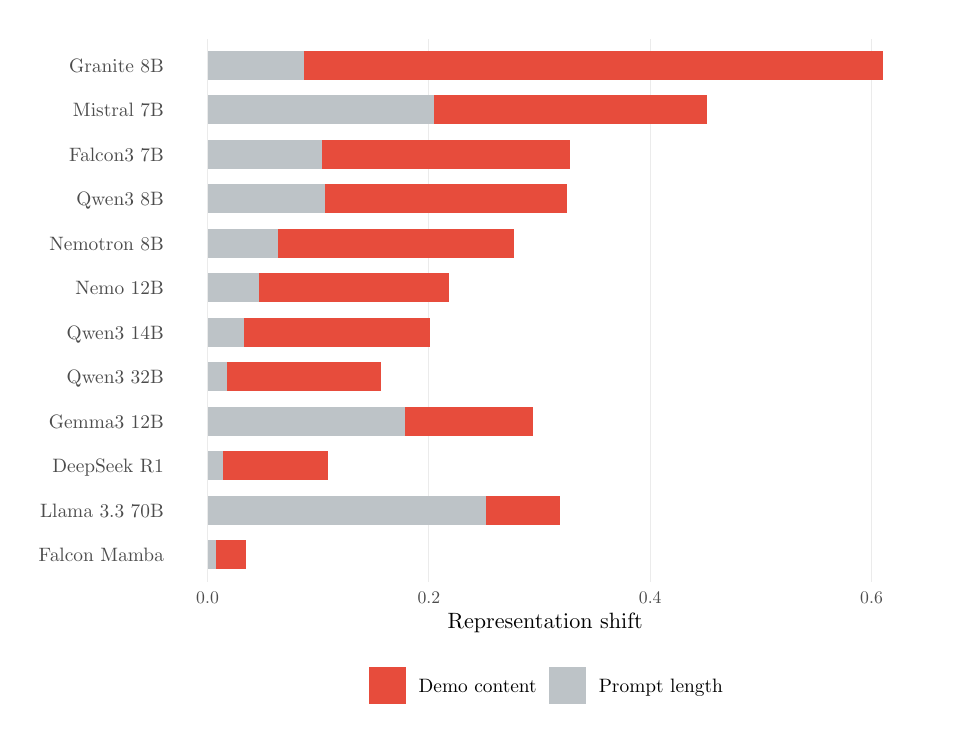
\begin{tikzpicture}[x=1pt,y=1pt]
\definecolor{fillColor}{RGB}{255,255,255}
\path[use as bounding box,fill=fillColor,fill opacity=0.00] (0,0) rectangle (325.21,252.94);
\begin{scope}
\path[clip] (  0.00,  0.00) rectangle (325.21,252.94);
\definecolor{fillColor}{RGB}{255,255,255}

\path[fill=fillColor] (  0.00,  0.00) rectangle (325.21,252.94);
\end{scope}
\begin{scope}
\path[clip] ( 52.80, 52.77) rectangle (321.21,248.94);
\definecolor{drawColor}{gray}{0.92}

\path[draw=drawColor,line width= 0.4pt,line join=round] ( 65.00, 52.77) --
	( 65.00,248.94);

\path[draw=drawColor,line width= 0.4pt,line join=round] (144.98, 52.77) --
	(144.98,248.94);

\path[draw=drawColor,line width= 0.4pt,line join=round] (224.96, 52.77) --
	(224.96,248.94);

\path[draw=drawColor,line width= 0.4pt,line join=round] (304.94, 52.77) --
	(304.94,248.94);
\definecolor{fillColor}{RGB}{189,195,199}

\path[fill=fillColor] ( 65.00,234.07) rectangle ( 99.71,244.52);
\definecolor{fillColor}{RGB}{231,76,60}

\path[fill=fillColor] ( 99.71,234.07) rectangle (309.01,244.52);
\definecolor{fillColor}{RGB}{189,195,199}

\path[fill=fillColor] ( 65.00,217.99) rectangle (146.86,228.44);
\definecolor{fillColor}{RGB}{231,76,60}

\path[fill=fillColor] (146.86,217.99) rectangle (245.31,228.44);
\definecolor{fillColor}{RGB}{189,195,199}

\path[fill=fillColor] ( 65.00,201.91) rectangle (106.31,212.36);
\definecolor{fillColor}{RGB}{231,76,60}

\path[fill=fillColor] (106.31,201.91) rectangle (195.80,212.36);
\definecolor{fillColor}{RGB}{189,195,199}

\path[fill=fillColor] ( 65.00,185.83) rectangle (107.35,196.28);
\definecolor{fillColor}{RGB}{231,76,60}

\path[fill=fillColor] (107.35,185.83) rectangle (194.76,196.28);
\definecolor{fillColor}{RGB}{189,195,199}

\path[fill=fillColor] ( 65.00,169.75) rectangle ( 90.43,180.20);
\definecolor{fillColor}{RGB}{231,76,60}

\path[fill=fillColor] ( 90.43,169.75) rectangle (175.65,180.20);
\definecolor{fillColor}{RGB}{189,195,199}

\path[fill=fillColor] ( 65.00,153.67) rectangle ( 83.59,164.12);
\definecolor{fillColor}{RGB}{231,76,60}

\path[fill=fillColor] ( 83.59,153.67) rectangle (152.42,164.12);
\definecolor{fillColor}{RGB}{189,195,199}

\path[fill=fillColor] ( 65.00,137.59) rectangle ( 78.23,148.04);
\definecolor{fillColor}{RGB}{231,76,60}

\path[fill=fillColor] ( 78.23,137.59) rectangle (145.38,148.04);
\definecolor{fillColor}{RGB}{189,195,199}

\path[fill=fillColor] ( 65.00,121.51) rectangle ( 71.96,131.96);
\definecolor{fillColor}{RGB}{231,76,60}

\path[fill=fillColor] ( 71.96,121.51) rectangle (127.58,131.96);
\definecolor{fillColor}{RGB}{189,195,199}

\path[fill=fillColor] ( 65.00,105.43) rectangle (136.46,115.88);
\definecolor{fillColor}{RGB}{231,76,60}

\path[fill=fillColor] (136.46,105.43) rectangle (182.77,115.88);
\definecolor{fillColor}{RGB}{189,195,199}

\path[fill=fillColor] ( 65.00, 89.35) rectangle ( 70.40, 99.80);
\definecolor{fillColor}{RGB}{231,76,60}

\path[fill=fillColor] ( 70.40, 89.35) rectangle (108.59, 99.80);
\definecolor{fillColor}{RGB}{189,195,199}

\path[fill=fillColor] ( 65.00, 73.27) rectangle (165.69, 83.72);
\definecolor{fillColor}{RGB}{231,76,60}

\path[fill=fillColor] (165.69, 73.27) rectangle (192.36, 83.72);
\definecolor{fillColor}{RGB}{189,195,199}

\path[fill=fillColor] ( 65.00, 57.19) rectangle ( 67.96, 67.64);
\definecolor{fillColor}{RGB}{231,76,60}

\path[fill=fillColor] ( 67.96, 57.19) rectangle ( 78.91, 67.64);
\end{scope}
\begin{scope}
\path[clip] (  0.00,  0.00) rectangle (325.21,252.94);
\definecolor{drawColor}{gray}{0.30}

\node[text=drawColor,anchor=base east,inner sep=0pt, outer sep=0pt, scale=  0.70] at ( 49.20, 60.01) {Falcon Mamba};

\node[text=drawColor,anchor=base east,inner sep=0pt, outer sep=0pt, scale=  0.70] at ( 49.20, 76.09) {Llama 3.3 70B};

\node[text=drawColor,anchor=base east,inner sep=0pt, outer sep=0pt, scale=  0.70] at ( 49.20, 92.17) {DeepSeek R1};

\node[text=drawColor,anchor=base east,inner sep=0pt, outer sep=0pt, scale=  0.70] at ( 49.20,108.25) {Gemma3 12B};

\node[text=drawColor,anchor=base east,inner sep=0pt, outer sep=0pt, scale=  0.70] at ( 49.20,124.33) {Qwen3 32B};

\node[text=drawColor,anchor=base east,inner sep=0pt, outer sep=0pt, scale=  0.70] at ( 49.20,140.41) {Qwen3 14B};

\node[text=drawColor,anchor=base east,inner sep=0pt, outer sep=0pt, scale=  0.70] at ( 49.20,156.49) {Nemo 12B};

\node[text=drawColor,anchor=base east,inner sep=0pt, outer sep=0pt, scale=  0.70] at ( 49.20,172.57) {Nemotron 8B};

\node[text=drawColor,anchor=base east,inner sep=0pt, outer sep=0pt, scale=  0.70] at ( 49.20,188.65) {Qwen3 8B};

\node[text=drawColor,anchor=base east,inner sep=0pt, outer sep=0pt, scale=  0.70] at ( 49.20,204.73) {Falcon3 7B};

\node[text=drawColor,anchor=base east,inner sep=0pt, outer sep=0pt, scale=  0.70] at ( 49.20,220.81) {Mistral 7B};

\node[text=drawColor,anchor=base east,inner sep=0pt, outer sep=0pt, scale=  0.70] at ( 49.20,236.89) {Granite 8B};
\end{scope}
\begin{scope}
\path[clip] (  0.00,  0.00) rectangle (325.21,252.94);
\definecolor{drawColor}{gray}{0.30}

\node[text=drawColor,anchor=base,inner sep=0pt, outer sep=0pt, scale=  0.64] at ( 65.00, 44.76) {0.0};

\node[text=drawColor,anchor=base,inner sep=0pt, outer sep=0pt, scale=  0.64] at (144.98, 44.76) {0.2};

\node[text=drawColor,anchor=base,inner sep=0pt, outer sep=0pt, scale=  0.64] at (224.96, 44.76) {0.4};

\node[text=drawColor,anchor=base,inner sep=0pt, outer sep=0pt, scale=  0.64] at (304.94, 44.76) {0.6};
\end{scope}
\begin{scope}
\path[clip] (  0.00,  0.00) rectangle (325.21,252.94);
\definecolor{drawColor}{RGB}{0,0,0}

\node[text=drawColor,anchor=base,inner sep=0pt, outer sep=0pt, scale=  0.80] at (187.01, 36.01) {Representation shift};
\end{scope}
\begin{scope}
\path[clip] (  0.00,  0.00) rectangle (325.21,252.94);
\definecolor{fillColor}{RGB}{231,76,60}

\path[fill=fillColor] (123.32,  8.52) rectangle (136.74, 21.94);
\end{scope}
\begin{scope}
\path[clip] (  0.00,  0.00) rectangle (325.21,252.94);
\definecolor{fillColor}{RGB}{189,195,199}

\path[fill=fillColor] (188.44,  8.52) rectangle (201.86, 21.94);
\end{scope}
\begin{scope}
\path[clip] (  0.00,  0.00) rectangle (325.21,252.94);
\definecolor{drawColor}{RGB}{0,0,0}

\node[text=drawColor,anchor=base west,inner sep=0pt, outer sep=0pt, scale=  0.70] at (141.26, 12.82) {Demo content};
\end{scope}
\begin{scope}
\path[clip] (  0.00,  0.00) rectangle (325.21,252.94);
\definecolor{drawColor}{RGB}{0,0,0}

\node[text=drawColor,anchor=base west,inner sep=0pt, outer sep=0pt, scale=  0.70] at (206.38, 12.82) {Prompt length};
\end{scope}
\end{tikzpicture}
